\section{Posición vehicular relativa}\label{apendice:posicion_relative}
La posición vehicular relativa se refiere a en qué lado de un vehículo A se encuentra
un vehículo B. Es decir, si se toma como referencia el primer vehículo, en qué lado se
encuentra el segundo; derecha, izquierda, delante o detrás.

El sistema de coordenadas GPS emplea un sistema diferente del cartesiano; el ángulo 0
comienza donde en el sistema tradicional (cartesiano) serían 90º. Además, en vez de ir
aumentando los grados de forma antihoraria lo hace al contrario, es decir, aumenta los
grados en sentido horario [Figura \ref{figure:rumbo_gps}].

El heading representa la dirección hacia la que un vehículo se está moviendo, empleando
el norte (0º) como referencia. Esta información, junto con la latitud, longitud y
altitud (Alt.) de los ciclistas y vehículos, es obtenida a través del GPS. Primero, se
calcula el ángulo existente entre los dos vehículos tomando como referencia al ciclista,
con esto se obtiene la posición del vehículo sin tener en cuenta la dirección hacia la que
circula el ciclista. Seguidamente, se relacionan el heading del ciclista y el ángulo entre
los dos vehículos para obtener el ángulo relativo entre ambos. Es decir, el ángulo respecto
la posición y dirección del ciclista, y la posición del vehículo. Finalmente, si el ángulo
relativo se encuentra entre 15º y 345º, se considera que está delante; entre 120º y 230º,
se encuentra detrás de su posición; entre 15º y 120º se considera que está a su derecha;
y entre 230º y 345º, a su izquierda. Estos cálculos son realizados en cada vehículo. En la
figura \ref{figure:demo_pos_relativa} se muestra un ejemplo del funcionamiento del algoritmo
en un entorno real.

El funcionamiento del algoritmo \ref{alg:relative_vehicular_pos} se puede resumir de la
siguiente forma:
\begin{enumerate}
	\item Calcular el ángulo existente entre los dos vehículos, sin tener en cuenta
	la dirección del primer vehículo.
	\item Se resta el heading del vehículo de referencia, al ángulo que hay entre
	los dos vehículos.
	\item Se contrasta con una serie de casos ya conocidos, y se devuelve el ángulo
 	relativo.
\end{enumerate}

\begin{listing}
	\begin{minipage}{.4\textwidth}
		\begin{minted}[linenos=true]{javascript}
function calcularPosicionRelativa(heading, oLatitude, oLongitude, pLatitude, pLongitude) {
  var degrees = calculateAngleBetweenTwoPoints(oLatitude, oLongitude, pLatitude, pLongitude);
  var relativeAngle = correctDegrees(degrees - heading);

  if (relativeAngle <= 15 && >= 0 || relativeAngle >= 345 && relativeAngle < 360) {
    return "FRONT";
  } else if (relativeAngle >= 120 && relativeAngle <= 230) {
    return "BACK";
  } else if (relativeAngle < 120 && relativeAngle > 15) {
    return "RIGHT";
  } else {
    return "LEFT";
  }
}

function calcularAnguloEntreDosPuntos(ox, oy, x, y) {
  return toDegrees(Math.atan2(y - oy, x - ox));
}
		\end{minted}
	\end{minipage}
	\caption{Cálculo de la posición relativa vehicular.}\label{alg:relative_vehicular_pos}
\end{listing}

\begin{figure}[H]
		\begin{center}
			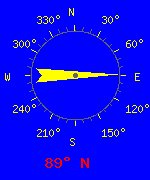
\includegraphics[scale=0.7]{bearing-1427303542791}
			\caption{Rumbo: el ángulo 0º está desplazado 90º con respecto al eje cartesiano.}
			\label{figure:rumbo_gps}
		\end{center}
\end{figure}
\begin{figure}[H]
		\begin{center}
			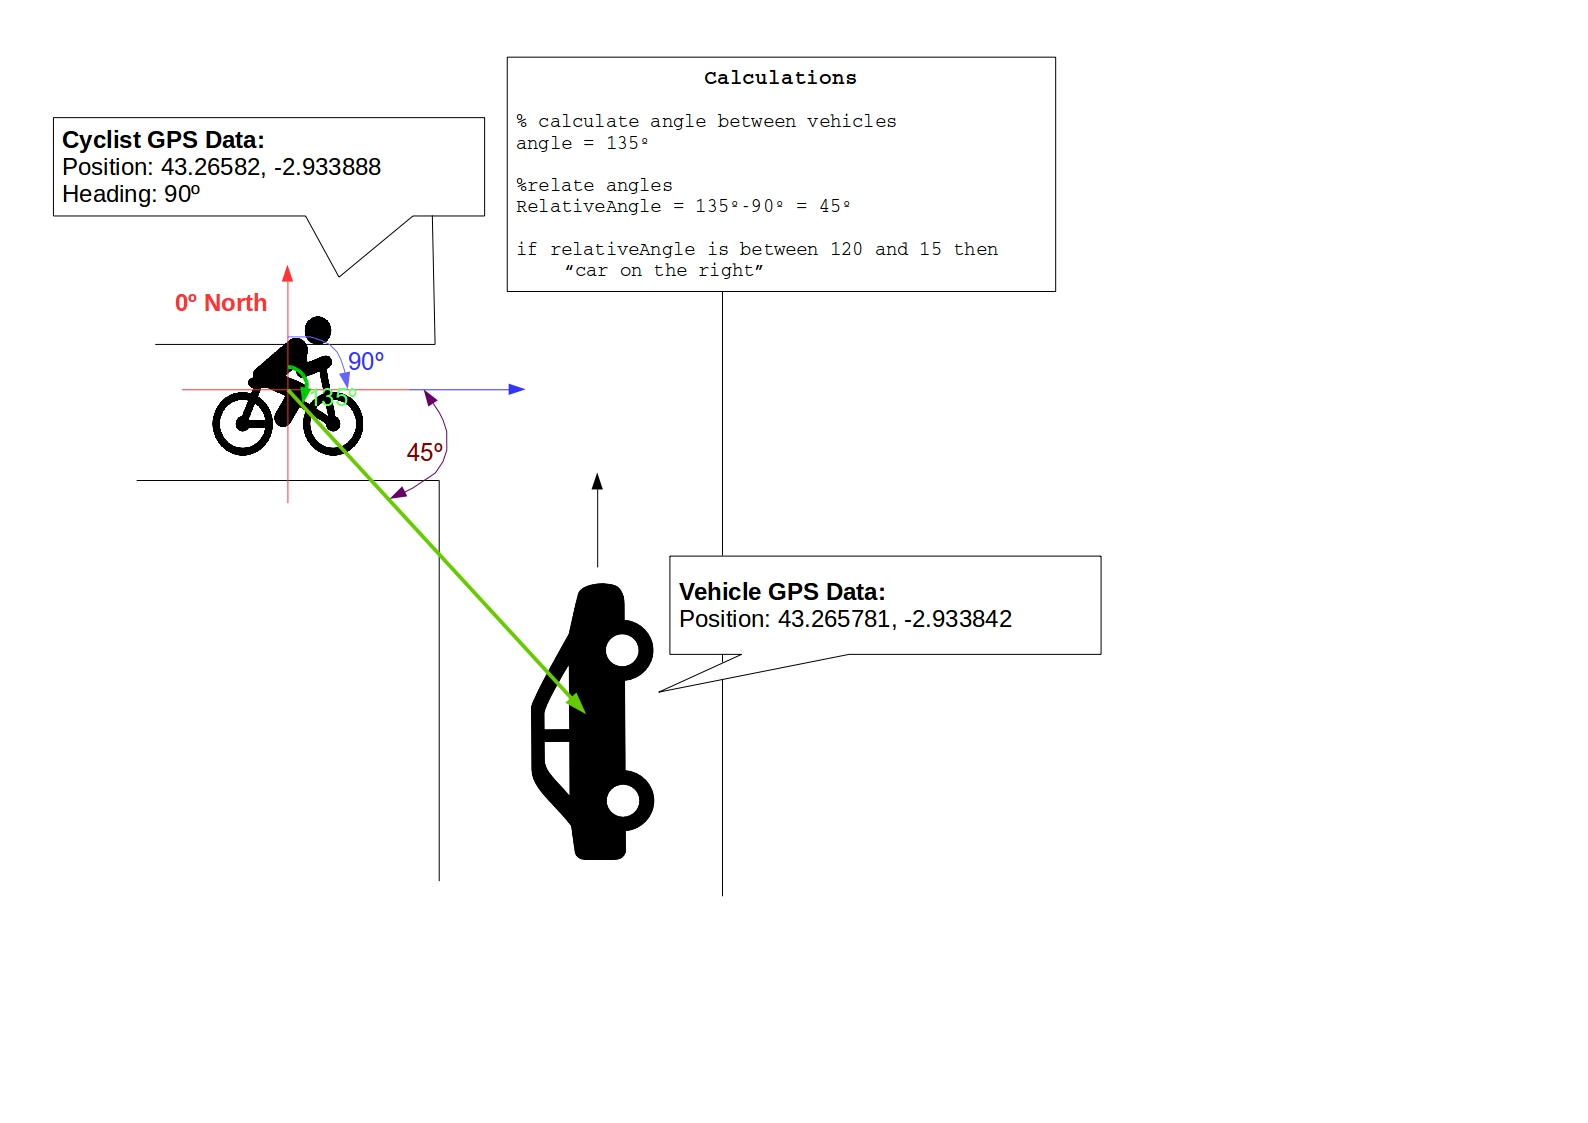
\includegraphics[scale=0.3]{demo-pos-relativa}
			\caption{Posición relativa vehicular.}
			\label{figure:demo_pos_relativa}
		\end{center}
\end{figure}

\subsection{Previsor de accidentes}
El algoritmo de posición vehicular relativa por sí solo no es suficiente para detectar
cuándo dos vehículos pueden encontrarse, tan solo prevé por dónde se puede encontrar
un vehículo. Por lo que para detectar una posible colisión es necesario un algoritmo
que emplee la posición vehicular relativa, la distancia entre los dos vehículos y el
sentido en que circulan ambos.

Mediante el algoritmo \ref{alg:deteccion_colisiones} se detecta si dos vehículos pueden
cruzarse en un rango de distancia especificado. Para ello, se requiere la posición de
ambos vehículos y la dirección hacia la que circulan. Se aplica un algoritmo para calcular
la nueva posición de ambos vehículos en el rango de distancia que se desee. Con las cuatro
posiciones obtenidas, primero se calcula si existe un punto de intersección, entre las dos
rectas. Finalmente, se comprueba si las rectas cortan entre las posiciones hacia la que se
dirigen los vehículos.

\begin{listing}
	\begin{minipage}{.4\textwidth}
		\begin{minted}[linenos=true]{javascript}
function isCollisionDanger(headingA, latitudeA, longitudeA, headingB, latitudeB, longitudeB) {
  var coord1 = movePosition(latitudeA, longitudeA, headingA);
  var coord2 = movePosition(latitudeB, longitudeB, headingB);
  var line1 = [[ latitudeA, longitudeA ], [ coord1.latitude, coord1.longitude ]];
  var line2 = [[ latitudeB, longitudeB ], [ coord2.latitude, coord2.longitude ]];

  var x1 = line1[0][0], y1 = line1[0][1] x2 = line1[1][0], y2 = line1[1][1];
  var x3 = line2[0][0], y3 = line2[0][1], x4 = line2[1][0], y4 = line2[1][1];
	
  var x = ((x1 * y2 - y1 * x2) * (x3 - x4) - (x1 - x2) * (x3 * y4 - y3 * x4))
    / ((x1 - x2) * (y3 - y4) - (y1 - y2) * (x3 - x4));
  var y = ((x1 * y2 - y1 * x2) * (y3 - y4) - (y1 - y2) * (x3 * y4 - y3 * x4))
	/ ((x1 - x2)*(y3 - y4) - (y1 - y2) * (x3 - x4));
	
  if (isNaN(x) || isNaN(y)) {
    return false;
  } else {
    if (x1 >= x2) {
      if (!(x2 <= x && x <= x1))
        return false; 
      else if (!(x1 <= x && x <= x2))
        return false; 

      if (y1 >= y2) {
        if (!(y2 <= y && y <= y1))
          return false;
      } else {
        if (!(y1 <= y && y <= y2))
          return false;
      }
    }
  }

  if (x3 >= x4) {
	if (!(x4 <= x && x <= x3)) 
	  return false;
  } else {
    if (!(x3 <= x && x <= x4)) 
      return false;
  }

  if (y3 >= y4) {
    if (!(y4 <= y && y <= y3))
      return false;
  } else {
    if (!(y3 <= y && y <= y4)) 
      return false;
  }

  return true;	
}
	\end{minted}
\end{minipage}
\caption{Algoritmo de previsión de colisiones.}\label{alg:deteccion_colisiones}
\end{listing}